\chapter{Abstraktiver Ansatz}
\thispagestyle{fancy}
\label{chap:Abstraktiver Ansatz}

\noindent
Unter Kenntnis der Grundlagen des \ac{DL} und des \ac{NLP} wird nun eine Architektur konzipiert und beschrieben, welche die \ac{ATS} gemäß des abstraktiven Ansatzes ermöglicht. Hierfür werden verschiedene Experimente durchgeführt, deren Training stets auf der beschriebenen Datengrundlage erfolgt.\\


\section{Metriken}
\noindent
Zuvor sind ausgewählte Metriken offenzulegen, mit denen die Qualität der \ac{ATS} gemessen werden kann: \ac{ROUGE} und \ac{BLEU}. In der Wissenschaft werden \ac{ATS}-Modelle meist mithilfe des \ac{ROUGE}-Scores evaluiert und verglichen. Dabei erfordern diese Metriken eine \ac{REFZ} zu jeder \ac{SYSZ}, welche maschinell generiert wurde. Dies ist unabhängig davon, ob das Training überwacht oder unüberwacht durchgeführt wurde. Allgemein unterliegen diese Metriken der Herausforderung, dass es für einen gegebenen Text keine objektiv beste Zusammenfassung gibt. Folglich können verschiedene \ac{SYSZ} oder sogar \ac{REFZ} gleich gut sein. Dies ist statistisch sehr schwer zu bewerten, zumal selbst Menschen aufgrund ihrer subjektiven Bewertungsweise nicht einheitlich definieren können, welche Faktoren für eine gute Zusammenfassung stehen. Weiterhin werden in den Metriken menschliche Bewertungsfaktoren wie beispielsweise Lesbarkeit nicht berücksichtigt \cite{LEM20}.\\


\subsection{ROUGE}
\noindent
\ac{ROUGE} kann zunächst mithilfe folgender Kennzahlen weitergehend differenziert werden: Recall, Precision und Measure. Dabei quantifiziert der Recall-Score den Anteil der sowohl in \ac{REFZ} als auch in \ac{SYSZ} vorkommender Wörter gemäß folgender Formel:\\
$$\frac{\text{Anzahl übereinstimmender Wörter}}{\text{Anzahl der Wörter in der REFZ}}$$
\newpage

\noindent
Sei hierfür verkürzt \glqq Der Sommer war sehr warm\grqq{} als \ac{REFZ} und \glqq Der Sommer war wieder sehr warm\grqq{} als \ac{SYSZ} gegeben. Dann gilt: $\text{Recall} = \frac{5}{5} = 1.0$. Trotzdem sollen \ac{SYSZ} nicht unendlich lang werden, um alle Wörter der \ac{REFZ} abzudecken, sondern weiterhin den eigentlichen Sinn einer Zusammenfassung erfüllen. Hier quantifiziert der Precision-Score den Anteil der tatsächlich relevanten Wörter gemäß folgender Formel:\\
$$\frac{\text{Anzahl übereinstimmender Wörter}}{\text{Anzahl der Wörter in der SYSZ}}$$ \newline

\noindent
Wie man sieht, ändert sich nur der Nenner. Im oben genannten Beispiel gilt somit: $\text{Precision} = \frac{5}{6} = 0.8\overline{3}$. Nimmt man ferner \glqq Der letzte Sommer war wieder sehr warm und trocken\grqq{} als neue \ac{SYSZ} an, dann reduziert sich der Precision-Score aufgrund der erhöhten Anzahl unrelevanter Wörter wie folgt: $\text{Precision} = \frac{5}{9} = 0.5\overline{5}$. Weiterhin kann der Measure-Score als gewöhnlicher F-Score verstanden und interpretiert werden. Er ergibt sich als harmonisches Mittel zwischen dem Recall und der Precision, womit er beide Scores berücksichtigt \cite[S.~1-3]{LIN04}.\\

\noindent
\ac{ROUGE} wird allgemein auch als \ac{ROUGE}-N geschrieben, wobei das N bestimmt, ob obige Kennzahlen auf Grundlagen von Uni-, Bi- oder Trigrammen berechnet werden sollen. Im genannten Beispiel wurden also die \ac{ROUGE}-1 Recall-, Precision- und Measure-Scores berechnet. Zudem existieren Ansätze, welche die \ac{LCS} verfolgen. Diese werden hier jedoch vernachlässigt.\\

\noindent
Trotz oder gerade wegen der wissenschaftlichen Verbreitung des \ac{ROUGE}-Scores kommt immer mehr Kritik auf. Demnach kann \ac{ROUGE} beispielsweise nicht zwischen verschiedenen aber bedeutungsähnlichen Wörtern unterscheiden. Dies führt tendenziell zu einer schlechteren Bewertung, obgleich ein gegebener Text etwa in einer entsprechenden \ac{SYSZ} präzise zusammengefasst wurde. Außerdem wird den Texten zur Berechnung des \ac{ROUGE}-Scores Kleinschreibung abverlangt, unabhängig von den vorgeschalteten Modellen. Die Bewertung geschieht also eher auf syntaktischer als auf semantischer Basis. Aufgrund der bereits genannten weitreichenden Nutzung des \ac{ROUGE}-Scores und der damit gegebenen Vergleichbarkeit kommt er trotzdem in dieser Arbeit zum Einsatz \cite[S.~5]{LIN04}.
\newpage

	
\subsection{BLEU}
\noindent
\ac{BLEU} kommt der Funktionsweise von \ac{ROUGE} weitestgehend gleich. Demnach repräsentiert der Score ebenfalls die Ähnlichkeit längendefinierter N-Gramme. Dabei wird weiterhin für jede \ac{SYSZ} eine entsprechende \ac{REFZ} gefordert. Beide Metriken funktionieren indes sprachunabhängig. Im Unterschied zu \ac{ROUGE} führt \ac{BLEU} einen multiplikativen Bestrafungsterm ein, um zu kurze \ac{SYSZ} zu entwerten. Dies ist nicht notwendig, wenn die \ac{SYSZ} länger ist als die \ac{REFZ}. Der Precision-Score berücksichtigt dies bereits \cite[S.~5]{PAP02}.\\

\noindent
Obgleich der \ac{BLEU}-Score primär die Bewertung von Übersetzungen unterstützt, eignet er sich gewissermaßen auch für \ac{ATS}-Aufgaben. Zuletzt konnte wissenschaftlich bewiesen werden, dass der \ac{BLEU}-Score recht gut mit menschlichen Bewertungen korreliert. Trotz ähnelnden Nachteilen zu denen des \ac{ROUGE}-Score wird auch der \ac{BLEU}-Score vergleichend in dieser Arbeit verwendet \cite[S.~6-7]{PAP02}.


\section{Architektur}
\noindent
Die Architektur ist als Sequence-to-Sequence-Transformer-Modell zu verstehen. Dabei wird sowohl der Encoder als auch der Decoder durch ein eigenständiges gemäß \ac{TL} vortrainiertes Modell repräsentiert. Aufgrund der bereits beschriebenen Grundlagen werden nun weitergehende Besonderheiten spezifiziert. Hierbei gibt es unter anderem die folgenden beiden Möglichkeiten, um den Encoder und den Decoder zu initialisieren \cite[S.~2]{ROT20}.\\

\noindent
Einerseits ist es möglich, den Encoder und den Decoder jeweils mit einem autarken Modell zu initialisieren, beispielsweise den Encoder mit \ac{BERT} und den Decoder mit \ac{GPT}. Andererseits ist es aber auch möglich, sowohl den Encoder als auch den Decoder mit dem gleichen Checkpoint eines Modells zu initialisieren, welches ursprünglich nur als Encoder trainiert wurde, beispielsweise mit \ac{BERT}. Aufgrund der Verfügbarkeit von \ac{BERT} wird in der Folge nur letztere Möglichkeit betrachtet. Die folgenden Ausführungen sind in \autoref{pic:EncoderDecoderBert} visualisiert \cite[S.~2-3]{ROT20}.
\newpage

\begin{figure}[h!]
  \centering
  \fbox{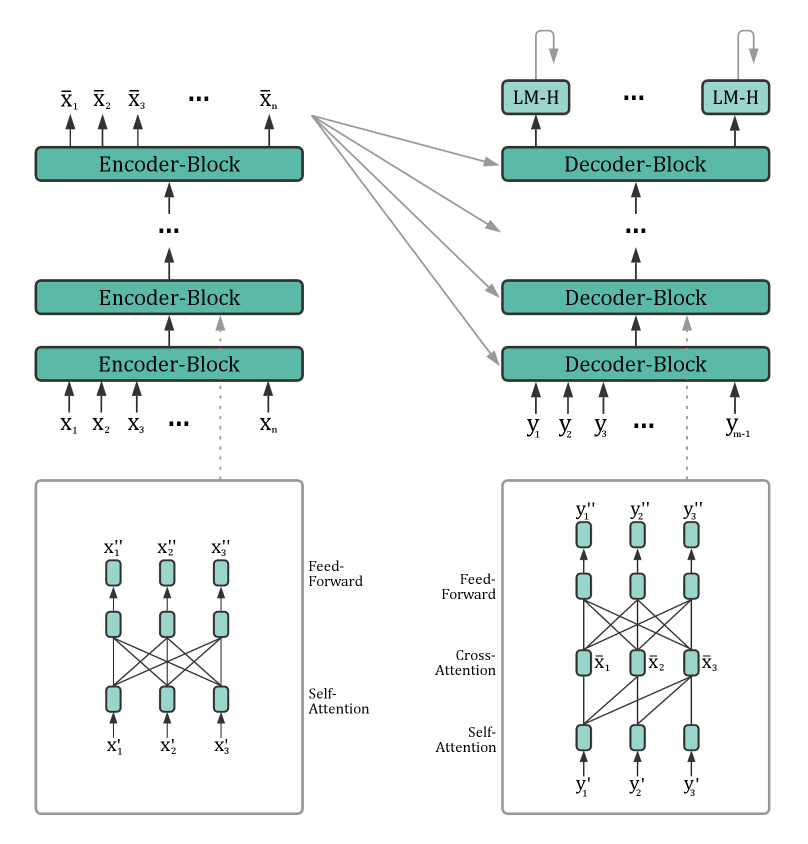
\includegraphics[width=0.85\linewidth]{./source/images/encoderdecoderbert.png}}
  \caption{Sequence-to-Sequence-Transformer-Modell mit BERT \cite{VON20}.}
  \label{pic:EncoderDecoderBert}
\end{figure}

\noindent
Die Gewichte der bidirektionalen Self-Attention-Schichten und der Feed-Forward-Schichten aller \ac{BERT}-Blöcke werden mit den vortrainierten Gewichten von \ac{BERT} initialisiert. Dabei kann der Encoder schlichtweg als \ac{BERT} in seiner bekannten Funktionsweise verstanden werden. Der Decoder hingegen bedarf mindestens der nachstehenden Anpassungen \cite{VON20}.\\

\noindent
Zunächst werden sogenannte Cross-Attention-Schichten zwischen den Self-Attention-Schichten und den Feed-Forward-Schichten aller \ac{BERT}-Blöcke eingeführt, um die kontextbasierten Sequenzen verarbeiten zu können. Die Gewichte der Cross-Attention-Schichten werden hierbei zufällig initialisiert \cite{VON20}.
\newpage

\noindent
Zudem werden die bidirektionalen Self-Attention-Schichten zu unidirektionalen Self-Attention-Schichten transformiert, um der autoregressiven Funktionsweise eines Decoders gerecht zu werden. Beide basieren auf den gleichen Projektionen aus Key, Query und Value, weshalb die Gewichte dieser Schichten weiterhin mit den Werten von \ac{BERT} initialisiert werden können. Die unidirektionalen Self-Attention-Schichten berücksichtigen nun nur noch vorangegangene Token, nicht mehr auch die nachstehenden Token. Dies führt interessanterweise zu veränderten Ausgabevektoren im Vergleich zum ursprünglich \ac{BERT}, obwohl sie die gleichen Gewichte teilen \cite[S.~2]{ROT20}.\\

\noindent
Zuletzt wird dem Decoder eine sogenannte Language-Model-Head-Schicht hinzugefügt, dessen Gewichte mit denen des gewählten Word Embeddings initialisiert werden. Hierbei handelt es sich erneut um \ac{BERT}. Es wird deutlich, dass sich der Encoder und der Decoder viele Gewichte teilen können. Dies führt zu einer erheblichen Reduktion des Speicherbedarfs, während die Qualität anschließender \ac{NLP}-Aufgaben nahezu unverändert bleibt \cite[S.~2]{ROT20}.\\

\noindent
Die Textinhalte der Datengrundlage bedürfen keiner weitergehenden Vorverarbeitung im herkömmlichen Sinne. Diese ist bekanntermaßen sehr individuell und stark modellabhängig. Unter Verwendung der als sehr robust geltenden Transformer-Architekturen entfällt daher die sonst übliche Textbereinigung sowie die Textnormalisierung. Dies unterliegt der Annahme, dass Transformer-Architekturen potenziell aus jeder Eigenart ein relevantes Feature schaffen können, welches das spätere Ergebnis begünstigt. Von der zugeführten Interpunktion und den vielfältigen Wortformen wird sich indes erhofft, potenzielle Mehr- oder Uneindeutigkeiten zu minimieren. Das Fine-Tuning sollte darüber hinaus unter gleichen Bedingungen wie das initiale Training stattfinden. Gleichzeitig sinkt hierdurch der vorverarbeitende Aufwand und damit auch etwaige Wartezeiten bei der praktischen Anwendung bereits trainierter Modelle in Echtzeit. Dennoch ist es möglich, bestimmte Vorverarbeitungsschritte a posteriori zu implementieren. Die Auswirkungen auf das Modell und die entsprechenden Ergebnisse würden somit zugleich messbar.\\

\noindent
TODO: Tokenizer auswählen, ebenfalls BERT, aber in der Cased-Version, Textlängen in den Korpora aufgreifen, aber Annahme anfügen, dass wichtige Informationen meist am Anfang der Texte stehen, sonst sind andere Operationen notwendig, bspw. Sliding-Window-Approach o.ä., BERT ist limitiert auf eine Tokenlänge von 512, was unter der Annahme akzeptiert wird, 128 wird als maximale Tokenlänge für die Zusammenfassung gewählt, weitere Parameter wie u.a. Batch Size nennen, auf tie_encoder_decoder, max_length (enc/ dec), vocab_size eingehen, Eignung von Python für ML/ DL beschreiben, Verwendung von CUDA und Torch erläutern, ggf. erst in den Experimenten, auch Seq2Seq-Klassen von HuggingFace sowie deren Parametrisierung erläutern, evtl. Longformer bzgl. der Behandlung längerer Token erwähnen, Aufbau von BERT und BERT.config aus dem Colab aufgreifen, ggf. einen Auszug dokumentieren, Quelle: \cite{VON20}, Daten und Baseline (SOTA, also englisches Modell reproduzieren) aufsetzen, dann Experimente anschließen, bzgl. Austausch vortrainierter Modelle, andere Versionen von BERT.\\

\noindent
+ \cite{VAS17}
+ \cite{NIT19} ab Kapitel 4
+ \url{https://huggingface.co/blog/how-to-generate}
+ S. 2 in \url{https://arxiv.org/pdf/1910.10781.pdf}: BERT ist SOTA in 11 NLP-Tasks ohne Modifikationen, hohe Adaptionsfähigkeit, abgesehen von der aufgabenbezogenen Ausgabeschicht
+ S. 2 in \url{https://arxiv.org/pdf/1910.10781.pdf}: Komplexität der Berechnung von Self-Attention in Transformers, insb. BERT, skaliert quadratisch mit der Sequenzlänge, zudem etwas nachteilig, dass positionsbezogene Schemata gelernt werden, weshalb sehr viele Trainingsdaten erforderlich sind, bestenfalls verschiedener Art und Domäne
+ S. 2 in \url{https://proceedings.neurips.cc/paper/2020/file/96671501524948bc3937b4b30d0e57b9-Paper.pdf}: Herausforderung bei der Verarbeitung langer Texte: Die vortrainierten Modelle wurden auf Texten mit einer maximalen Sequenzlänge trainiert, bei BERT sind das 512 Token, d.h. Sequenzen werden nach 512 Token abgeschnitten, doch ein einfaches Erhöhen hilft nicht unbedingt, weil Speicher und Rechenzeit quadratisch ansteigen, Ansatz: Subtexte mit in Summe 512 Token extrahieren, Sliding Window Approach, wobei dabei langfristige Abhängigkeiten verloren gehen, Ansatz: Text alle 512 Token splitten, letzten Part padden, dann einzeln zusammenfassen und Zusammenfassungen konkatenieren
+ \url{https://arxiv.org/pdf/2007.14062.pdf}: Big Bird auch (s.o.)
+ S. 1 in \url{https://arxiv.org/pdf/2004.05150.pdf}: Longformer auch (s.o.), erreicht ebenfalls lineare Komplexität durch lokale Attention und einer angeschlossenen globalen Attention
+ S. 2: Aber: Keine multilingualen Modelle verfügbar, weil Forschung noch jung, daher weiterhin Standard-BERT, Anpassungen dann bei neuen Erkenntnissen
+ \url{https://towardsdatascience.com/deep-generative-models-25ab2821afd3}: Deep Generative Models: BERT: Verteilung von Daten unüberwacht lernen, d.h. ungelabelte Daten, Berechnung bedingter Wahrscheinlichkeiten
+ Laufzeitkomplexität durch Self-Attention (jedes Zeichen mit jedem Zeichen), zu aufwendig für Longformer o.ä., Attention-Mechanismen daher austauschen, bspw. lokale Attention, sonst Sliding-Window-Approach (512 Token vorne, mittig, hinten), sonst Ausblick, Literaturrecherche
+ YAN19 auf S. 1, ROT20 auf S. 2 rechts und S. 6 unten
+ Encoder zur NLU und Decoder zur NLG, d.h. BERT oder andere Transformer als vortrainiertes multilinguales Modell für Encoder/ Decoder nutzen
+ Warm-Start des Encoder-Decoder-Models, d.h. kein initiales Training erforderlich, welches im Bereich von NLP-Tasks ein Neuerlernen einer Sprache bedeuten würde, Encoder-Decoder-Weight-Sharing bei der Initialisierung nochmal schriftlich kompaktieren und deutlich machen
+ \cite{YAN19} S. 4 rechts, S. 5 oben für Evaluation, S. 6 links unten für Konfiguration.\\


\section{Experimente}
\noindent
+ Mit der Beschreibung des Trainings beginnen
+ ZIH-Cluster mit HPC/ Taurus aus IT- /ML-Infrastruktur zum Training, Spezifikationen etwas beschreiben, z.B. Tesla K80
+ Setup beschreiben \url{https://docs.aws.amazon.com/dlami/latest/devguide/tutorials.html}, \url{https://youtu.be/pK-LYoRwp-k?list=WL}
+ Vergleichstabelle der Experimente einbinden und beschreiben
+ Typisches Diagramm zur Visualisierung des Trainingsprozesses anfügen
+ Verhalten des Modells interpretieren und Anpassungen ableiten, bspw. Exploitation wegen der Struktur der Artikel nochmal aufgreifen, ggf. erst bei der sprachtechnischen Adaption.\\
